%!TEX root = ../Main.tex
\section{Size inference}
The array operations in a cluster are fused together into a loop with a specific number of iterations.
Array operations that process different sized arrays cannot usually be assigned to the same cluster, because they require different sized loops.
Consumers of arrays produced by size-changing operations can be assigned to the same cluster as operations that process different sized arrays, but only in specific circumstances, which we shall see in \cref{clustering/size/transducers}.
Before performing clustering, we need to infer the relative sizes of each array in the program, as the sizes determine the relative loop sizes of each array operation, and whether they can be assigned to the same cluster.
We use a simple constraint-based inference algorithm.
Size inference has been previously described in the context of array fusion by \citet{chatterjee1991size}.
In constrast to our algorithm, \citet{chatterjee1991size} does not support size-changing functions such as filter.

Although our constraint-based formulation of size inference is reminiscent of type inference for HM(X)~\cite{odersky1999type}, there are important differences.
Firstly, our type schemes include existential quantifiers, which express the fact that the sizes of arrays produced by filter operations are statically unknown, in general.
The output size of \Hs@generate@ is also statically unknown, as the result size is data-dependent and is not available until runtime.
HM(X) style type inferences use the $\exists$ quantifier to bind local type variables in constraints, and existential quantifiers do not appear in type schemes.
Secondly, our types are first-order only, as program graphs cannot take other program graphs as arguments.
Provided we generate the constraints in the correct form, solving them is straightforward.

Size inference cannot statically infer array sizes for all programs.
The $\Hs/map/_n$ combinator requires all input arrays to be the same size, and returns an output array of the same size.
Compared to \Hs/zipWith/, which returns a statically unknown size, this extra restriction gives size inference more information about the size of the output array, which in turn may allow more array operations to be assigned to the same cluster.
If we cannot statically determine that all input arrays given to $\Hs/map/_n$ are the same size, size inference will fail: the program may still be compiled, but fusion is not performed.

% -----------------------------------------------------------------------------
\begin{figure}
\begin{tabbing}
MMMMMMMMM \= MM  \= MM \= MMMMMM \= \kill
\textbf{Size Type}
\> $\tau$   \> @::=@  \> $k$                  \> (size variable)       \\
\>          \> $~|$   \> $\tau \times \tau$   \> (cross product)
\end{tabbing}

\begin{tabbing}
MMMMMMMMM \= MM  \= MM \= MMMMMM \= \kill
\textbf{Size Constraint}
\> $C$      \> @::=@  \> $\true$               \> (trivially true)      \\
\>          \> $~|$   \> $k = \tau$           \> (equality constraint) \\
\>          \> $~|$   \> $C \wedge C$         \> (conjunction)
\end{tabbing}

\begin{tabbing}
MMMMMMMMM \= MM  \= MM \= MMMMMM \= \kill
\textbf{Size Scheme}
\> $\sigma$ \> @::=@  
        \> $\forall \ov{k}.~ \exists \ov{k}.~ (\ov{ x : \tau }) \to (\ov{x : \tau})$
\end{tabbing}

\caption{Sizes, constraints and schemes}
\label{clustering:f:constraints}
\end{figure}


\newcommand{\constr}[1]{\llbracket #1 \rrbracket}


% -----------------------------------------------------------------------------
\subsection{Size types, constraints and schemes}
\label{clustering:s:SizeTypes}
\Cref{clustering:f:constraints} shows the grammar for size types, constraints and schemes.
A size scheme is like a type scheme from Hindley-Milner style type systems, except that it only mentions the size of each input array, and ignores the element types.

A size may either be a variable $k$ or a cross product of two sizes.
We use the latter to represent the result size of the \Hs@cross@ operator discussed in the previous section.
Constraints may either be trivially $\true$, an equality $k = \tau$, or a conjunction of two constraints $C \wedge C$.
We refer to the trivially true and equality constraints as \emph{atomic constraints}.
Size schemes relate the sizes of each input and output array.
The \Hs@normalize2@ example from \cref{clustering:f:normalize2-clusterings}, which returns two output arrays of the same size as the input, has the following size scheme:
% For example, the size scheme for the \Hs@normalize2@ example from \cref{clustering:f:normalize2-clusterings}, which returns two arrays of the same size as the input, is as follows:
$$
\Hs@normalize2@ ~:_s \forall k.~ (xs : k) \to (ys_1 : k,~ ys_2 : k)
$$

We write $:_s$ to distinguish size schemes from type schemes.

The existential quantifier appears in size schemes when the array produced by a filter or generate appears in the result.
For example:

\begin{haskell}
filterLeft %\(:\sb{s}\,\forall\,k\sb{1}.\,\exists\,k\sb{2}.\,(xs\,:\,k\sb{1})\;\to\;(ys\sb{1}\,:\,k\sb{1},\,ys\sb{2}\,:\,k\sb{2})\)%
filterLeft xs
  = let ys1 = map (+ 1)   xs
        ys2 = filter even xs
    in (ys1, ys2)
\end{haskell}

The size scheme of \Hs@filterLeft@ shows that it works for input arrays of all sizes.
The first result array has the same size as the input, and the second has some unrelated and unknown size.

Finally, note that size schemes form only one aspect of the type information that would be expressible in a full dependently typed language.
For example, in Coq or Agda we could write something like:

\begin{haskell}
filterLeft : %\(\forall\,k\sb{1}:\,\)Nat\(.~\,\exists\,k\sb{2}:\,\)Nat\(.\)% Array %\(k\sb{1}\)% Float -> (Array %\(k\sb{1}\)% Float, Array %\(k\sb{2}\)% Float)
\end{haskell}

However, the type inference systems for fully higher order dependently typed languages typically require quantified types to be provided by the user, and do not perform the type generalization process.
In our situation, we need automatic type generalization, but for a first-order language only.


%!TEX root = ../Main.tex

\begin{figure*}
\footnotesize
% -------------------------------------------------------------------
$$
\fbox{$
 \SizeL {\Gamma}
        {\textit{lets}}
        {\Gamma}
        {C}
$}
$$
%
$$
\ruleI{}{
        \SizeL  {\Gamma}
                {@let@ ~\cdot~ @in@~ exp}
                {\Gamma}
                {\true}
}
\quad
\textrm{(SNil)}
$$

$$
\ruleI  {\SizeB {\Gamma_1}
                {zs}
                {b}
                {\Gamma_2}
                {C_1}
         \quad
         \SizeL {\Gamma_2}
                {@let@~ bs~ @in@~ exp}
                {\Gamma_3}
                {C_2}
        }
        {\SizeL {\Gamma_1}
                {@let@~ zs~ = b~ ;~ bs~ @in@~ exp}
                {\Gamma_3}
                {C_1 \wedge C_2}
        }
\quad
\textrm{(SCons)}
$$

% -------------------------------------------------------------------
$$
\fbox{$ 
 \SizeB {\Gamma}
        {z}
        {bind}
        {\Gamma}
        {C}
$}
$$
%
$$
\begin{array}{lllll}
% map_n
\SizeB  {\Gamma[xs_i : k_i]^{i \gets 1..n}       &}
        {zs}
        {@map@_n~ f~ \{xs_i\}^{i \gets 1..n}     &}
        {\Gamma,~ zs : k_{zs},~ k'               &}
        {\bigwedge_{i \gets 1..n}
                \{k_i = k'\}
         ~\wedge~ k_{zs} = k'}
\\[1ex]

% filter
\SizeB  {\Gamma                                 &}
        {zs}
        {@filter@~ f~ xs                        &}
        {\Gamma,~ zs : k_{zs},~ \exists k'      &}
        {k_{zs} = k'}
\\[1ex]

% fold
\SizeB  {\Gamma                                 &}
        {x~}
        {@fold@~ f~ xs                          &}
        {\Gamma                                 &}
        {\true}
\\[1ex]

% generate
\SizeB  {\Gamma                                 &}
        {zs}
        {@generate@~ s~ f                       &}
        {\Gamma,~ zs : k_{zs},~ \exists k'      &}
        {k_{zs} = k'}
        \\[1ex]

% gather
\SizeB  {\Gamma[is : k_{is}]                    &}
        {zs}
        {@gather@~ xs~ is                       &}
        {\Gamma,~ zs : k_{zs},~ k'              &}
        {k_{zs} = k',~ k_{is} = k'}
\\[1ex]

% cross
\SizeB  {\Gamma[xs : k_{xs},~ ys : k_{ys}]      &}
        {zs}
        {@cross@~ xs~ ys                        &}
        {\Gamma,~ zs : k_{zs},~ k',~ k''        &}
        {k_{zs} = k' \times k'' 
                ~\wedge~ }
\\
& & & \quad\ \  k_{xs} = k' ~\wedge~ k_{ys} = k''
\\[1ex]

% external
\SizeB  {\Gamma                                 &}
        {zs}
        {@external@~ \{xs\}^{i \gets 1..n}      &}
        {\Gamma,~ zs : k_{zs},~ \exists k'      &}
        {k_{zs} = k'}
\end{array}
$$

\caption{Constraint generation for size inference}
\label{clustering:f:ConstraintGeneration}
\end{figure*}


% -----------------------------------------------------------------------------
\subsection{Constraint generation}
The rules for constraint generation are shown in \cref{clustering:f:ConstraintGeneration}.
The first judgment form is written as ($\SizeL{\Gamma_1}{\textit{lets}}{\Gamma_2}{C}$) and reads: ``under environment $\Gamma_1$, the bindings in $\textit{lets}$ produce the result environment $\Gamma_2$ and size constraints $C$''.
The judgment form ($\SizeB{\Gamma_1}{zs}{b}{\Gamma_2}{C}$) performs constraint generation for a single binding and reads: ``under environment~$\Gamma_1$, array variable $zs$ binds the result of $b$, producing a result environment $\Gamma_2$ and size constraints $C$''.
The environment ($\Gamma$) has the following grammar:
$$
\Gamma~ @::=@ ~~\cdot ~~|~~ \Gamma,~ \Gamma ~~|~~ zs : k ~~|~~ k ~~|~~ \exists k
$$

As usual, ($\cdot$) represents the empty environment and ($\Gamma,~ \Gamma$) represents environment concatenation.
The element ($zs : k$) records the size $k$ of some array variable $zs$.
A plain $k$ indicates that $k$ can be unified with other size types when solving constraints, whereas $\exists k$ indicates a  \emph{rigid} size variable that cannot be unified with other sizes.
We use the $\exists k$ syntax because this variable will also be existentially quantified if it appears in the size scheme of the overall program.

The constraints are generated in a specific form in \cref{clustering:f:ConstraintGeneration}, to facilitate the constraint solving process.
For each array variable in the program, we generate a new size variable, like size $k_{zs}$ for array variable $zs$.
These new size variables always appear on the \emph{left} of atomic equality constraints.
For each array binding, we may also introduce unification or rigid variables; these appear on the \emph{right} of atomic equality constraints.

The final environment and constraints generated for the \Hs@normalize2@ example from \cref{clustering:s:Introduction} are as follows, with the program shown on the right:

\begin{minipage}{0.5\textwidth}
$$
\begin{array}{ll}
   & @xs @ : k_{xs},~
\\ & @gts@ : k_{gts},~ \exists k_1,
\\ & @ys1@ : k_{ys1},~ k_2,
\\ & @ys2@ : k_{ys2},~ k_3
\\
\vdash & \true 
        ~\wedge~  k_{gts} = k_1
\\ \wedge & \true
        ~ \wedge~  k_{xs}  ~= k_2
        ~ \wedge~  k_{ys1}  = k_2 
\\     &~~~~~~~\; 
          \wedge~  k_{xs}   = k_3
        ~ \wedge~  k_{ys2}  = k_3
\end{array}
$$
\end{minipage}
\begin{minipage}{0.5\textwidth}
% normalize2 %\(:_s \forall k_{xs}.~ (xs : k_{xs}) \to (ys_1 : k_{xs},~ ys_2 : k_{xs})\)%
\begin{haskell}
normalize2 xs
 = let sum1 = fold   (+)  0   xs
       gts  = filter (>   0)  xs
       sum2 = fold   (+)  0   gts
       ys1  = map    (/ sum1) xs
       ys2  = map    (/ sum2) xs
   in (ys1, ys2)
\end{haskell}
\end{minipage}

To compute the constraints and environment for this example, the input environment given to constraint generation records that the input array \Hs/xs/ has the corresponding size type $k_{xs}$.
This input environment is described in \cref{clustering:s:ConstraintSolvingGen}.
For each binding, the rules in \cref{clustering:f:ConstraintGeneration} generate a constraint and add any required array and size bindings to the environment.
The \Hs/sum1/ binding, a \Hs/fold/, does not bind any array variables and works for any input size, so the corresponding rule leaves the environment as-is and produces a $\true$ constraint.
For the \Hs/gts/ binding, a \Hs/filter/, the size of the output array is unknown.
The \Hs/filter/ rule records the size of the output array by introducing a new size-type variable $k_{gts}$, as well as an existential variable $k_1$; the rule also generates the constraint ($k_{gts} = k_1$).
For the \Hs/ys1/ binding, a \Hs/map/, the size of the output array is the same as the input array.
The \Hs/map/ rule introduces a new size variable $k_{ys1}$ to record the size of the output array, and introduces a new unification variable $k_2$.
The rule introduces constraints requiring the new unification variable $k_2$ to be equal to both the input size variable $k_{xs}$ and the output size variable $k_{ys1}$.
In the constraints, array size variables occur on the left-hand side and unification variables occur on the right-hand side.
Constraint generation for the remaining bindings proceeds similarly.


% -------------------------------------------------------------------
\subsection{Constraint solving and generalization}
\label{clustering:s:ConstraintSolvingGen}
\Cref{clustering:f:ConstraintSolving} shows the rule for assigning a size scheme to a program.
The top-level judgment form ($\SizeF{\program}{\sigma}$) assigns size scheme $\sigma$ to $\program$.

%!TEX root = ../Main.tex

\newcommand\ins{\textit{ins}}
\newcommand\inty{\textit{inty}}
\begin{figure*}
\footnotesize
$$
\fbox{$
 \SizeF {\program}{\sigma}
$}
$$
$$
\ruleI  {
          \SizeL{\Gamma_0}
                {@let@~ bs~ @in@~ \{ ys_j \}^{j \gets 1 .. m}}
                {\Gamma_1}{C_1}
\qquad
  (\Gamma_2,C_2) = \textrm{SOLVE}(\Gamma_1,~ C_1)
  \qquad
          \forall k \in \textrm{fv}(\ov{s}).~
          (\exists k) \notin \Gamma_2
        }
        {
        \begin{array}{c}
        \SizeF{f~ \{xs\}^{i \gets 1..n}
                        = @let@~ bs~ @in@~ \{ys\}^{j \gets 1..m}
                }
                { \forall \overline{k_a}.~ 
                  \exists \overline{k_e}.~
                        (\{ xs_i : s_i \}^{i \gets 1..n}) \to
                        (\{ ys_j : t_j \}^{j \gets 1..m})
                }
\\[1em]
\begin{array}{lll}
\mbox{where }
  & \Gamma_0 & = \{k_i,~ xs_i : k_i \}^{ i \gets 1 .. n }
\\
\\
  & \ov{s} & = \{ s_i ~|~ i \in 1..n  ~\wedge~ (k_i = s_i) \in C_2 \}
\\
 & \ov{k'} & = \{ k'_j ~|~ j \in 1..m ~\wedge~ (ys_j : k_j') \in \Gamma_2 \}
\\
  & \ov{t} & = \{ t_j ~|~ j \in 1..m  ~\wedge~ (k_j' = t_j ) \in C_2 \}
\\
\\
 & \ov{k_a} & = \{ k ~|~ k         \in \Gamma_2 ~\wedge~ k \in \textrm{fv}(\ov{s}) \}  
%                        ~\cap~ (\bigcup_{i \gets 1 .. n}\textrm{fv}(s_i))
\\
 & \ov{k_e} & = \{ k ~|~ \exists k \in \Gamma_2 ~\wedge~ k \in \textrm{fv}(\ov{t}) \}
%                        ~\cap~ (\bigcup_{j \gets 1 .. m}\textrm{fv}(t_j))
\end{array}
\end{array}
        }
\quad
\textrm{(SProgram)}
$$

\caption{Constraint solving for size inference}
\label{clustering:f:ConstraintSolving}
\end{figure*}



Rule (SProgram) assigns a size scheme to a program by first extracting size constraints, before solving them and generalizing the result.
In the rule, $\Gamma_0$ is used as the input environment to constraint generation, and is constructed by generating a fresh size variable ($k_i$) for each input array ($xs_i$).
The environment and constraints produced by constraint generation are named $\Gamma_1$ and $C_1$; these constraints are then solved using the $\textrm{SOLVE}$ function, which we describe soon.
The constraints, after being solved, are stored in $C_2$, and the environment in $\Gamma_2$.
We use the solved constraints to find the size types of the input arrays ($\ov{s}$), and the size types of the output arrays ($\ov{t}$).
We perform generalization by adding universal quantifiers for the unification variables mentioned by the types of input arrays ($\ov{k_a}$), and adding existential quantifiers for the existential variables mentioned by the types of output arrays ($\ov{k_e}$).
Finally, we require that the types of input arrays do not mention any existential variables; an example of this restriction is shown in \cref{clustering:s:RigidSizes}.

In the rule, the solving process is indicated by $\textrm{SOLVE}$, and takes an environment and a constraint set, and produces a solved environment and constraint set.
As the constraint solving process is both standard and straightforward, we only describe it informally.

During constraint generation in the previous section, we were careful to ensure that all the size variables named after program variables are on the left of atomic equality constraints, while all the unification and existential variables are on the right.
To solve the constraints, we keep finding pairs of atomic equality constraints where the same variable appears on the left, unify the right of both of these constraints, and apply the resulting substitution to both the environment and original constraints.
When there are no more pairs of constraints with the same variable on the left, the constraints are in solved form and we are finished.

During constraint solving, all unification variables occuring in the environment can have other sizes substituted for them.
In contrast, the rigid variables marked by the $\exists$ symbol cannot.
For example, consider the constraints for \Hs@normalize2@ mentioned before:
$$
\begin{array}{ll}
   & @xs @ : k_{xs},~
@gts@ : k_{gts},~ \exists k_1,~
@ys1@ : k_{ys1},~ k_2,~
@ys2@ : k_{ys2},~ k_3
\\
\vdash & \true 
        ~\wedge~  k_{gts} = k_1 ~\wedge~ \true
\\     &~~~~~~~\; 
          \wedge~  \colorbox{green!10}{$k_{xs}  ~= k_2$}
          \wedge~  k_{ys1}  = k_2 
\\     &~~~~~~~\; 
        ~ \wedge~  \colorbox{green!10}{$k_{xs}   = k_3$}
        ~ \wedge~  k_{ys2}  = k_3
\end{array}
$$

In the highlighted constraints, $k_{xs}$ is mentioned twice on the left of an atomic equality constraint, so we can substitute $k_2$ for $k_3$. Eliminating the duplicates, as well as the trivially $\true$ terms then yields:
$$
\begin{array}{ll}
   & @xs @ : k_{xs},~
@gts@ : k_{gts},~ \exists k_1,~
@ys1@ : k_{ys1},~ k_2,~
@ys2@ : k_{ys2},~ k_3
\\
\vdash & k_{gts} = k_1
        ~\wedge~  k_{xs}  ~= k_2
        ~\wedge~  k_{ys1}  = k_2 
        ~\wedge~  k_{ys2}  = k_2
\end{array}
$$

To produce the final size scheme, we look up the sizes of the input and output variables of the original program from the solved constraints and generalize appropriately.
This process is determined by the top-level rule in \cref{clustering:f:ConstraintSolving}.
In the case of \Hs/normalize2/, no rigid size variables appear in the result, so we can universally quantify all size variables to get the following size scheme:
$$\Hs@normalize2@ ~:_s \forall k_2. (xs : k_2) \to (ys_1 : k_2,~ ys_2 : k_2)
$$


Rule~(SProgram) also characterises the programs we accept: a program is \emph{valid} if and only if $\exists \sigma.\ \SizeF{\program}{\sigma}$. 

% -----------------------------------------------------------------------------
\subsection{Rigid sizes}
\label{clustering:s:RigidSizes}
When the environment of our size constraints contains rigid variables (indicated by $\exists k$), we introduce existential quantifiers instead of universal quantifiers into the size scheme.
Consider the \Hs@filterLeft@ program from \cref{clustering:s:SizeTypes}:
\begin{haskell}
filterLeft xs
 = let ys1 = map (+ 1)   xs
       ys2 = filter even xs
   in (ys1, ys2)
\end{haskell}

The size constraints for this program, already in solved form, are as follows:
$$
\begin{array}{ll}
       & xs : k_{xs},~ ys_1 : k_{ys1},~ k_1,~ ys_2 : k_{ys2},~ \exists k_2
\\
\vdash &          k_{xs}   = k_1
        ~\wedge~  k_{ys_1} = k_1 
        ~\wedge~  k_{ys_2} = k_2
\end{array}
$$

As variable $k_2$ is marked as rigid, we introduce an existential quantifier for it, producing the size scheme stated earlier:

$$
@filterLeft@ :\sb{s}\,\forall k\sb{1}.\ \exists k\sb{2}.\ (xs\,:\,k\sb{1})\;\to\;(ys\sb{1}\,:\,k\sb{1},\,ys\sb{2}\,:\,k\sb{2})
$$

Note that, although rule~(SProgram) from \cref{clustering:f:ConstraintSolving} performs a \emph{generalization} process, there is no corresponding instantiation rule.
The size inference process works on the entire graph at a time, and there is no mechanism for one operator to invoke another.
To say this another way, all subgraphs are fully inlined.
Recall from \cref{clustering:s:CombinatorNormalForm} that we assume our operator graphs are embedded in a larger host program.
We use size information to guide the clustering process, and although the host program can certainly call the operator graph, static size information does not flow across this boundary.

When producing size schemes, we do not permit the arguments of an operator graph to have existentially quantified sizes.
This restriction is necessary to reject programs that we cannot statically guarantee will be well-sized.
For example:
\begin{haskell}
bad1 xs
 = let flt = filter p xs
       ys  = map2   f flt xs
   in  ys
\end{haskell}

The above program filters its input array, and then applies \Hs@map2@ to the filtered version as well as the original array.
As the \Hs@map2@ operator requires both of its arguments to have the same size, \Hs@bad1@ would only be valid when the predicate \Hs@p@ is always true.
We could execute this program as a process network if we replaced the \Hs/map2/ operator with \Hs/zipWith/, and explicitly read from the input array \Hs/xs/ twice, as in the two-source version of \Hs/partitionAppend/ from \cref{s:Benchmarks:partitionAppend}.
The result size of the \Hs/zipWith/ operator is the smaller of the two input operators; the extra size restriction on \Hs/map2/ simplifies size inference, as we do not need to introduce the concept of the minimum of size types.
The size constraints for \Hs/bad1/ are as follows:
$$
\begin{array}{ll}
       & xs : k_{xs},~ \mi{flt} : k_{\mi{flt}},~ \exists k_1,~ ys : k_{ys},~ k_2
\\
\vdash &          k_{\mi{flt}}  = k_1
        ~\wedge~  k_{\mi{flt}}  = k_2
        ~\wedge~  k_{xs}   = k_2
        ~\wedge~  k_{ys}   = k_2
\end{array}
$$

Solving these constraints then yields:

$$
\begin{array}{ll}
       & xs : k_{xs},~ \mi{flt} : k_{\mi{flt}},~ \exists k_1,~ ys : k_{ys},~ k_1
\\
\vdash &          k_{\mi{flt}}  = k_1
        ~\wedge~  k_{xs}   = k_1
        ~\wedge~  k_{ys}   = k_1
\end{array}
$$

In this case, rule~(SProgram) does not apply, because the parameter variable $xs$ has size $k_1$, but $k_1$ is marked as rigid in the environment (with $\exists k_1$). 
This function is rejected by size inference, as a caller cannot guarantee that an input array's size matches the existential size type chosen by the function.

As a final example, the following program is ill-sized because the two filter operators are not guaranteed to produce the same number of elements:
\begin{haskell}
bad2 xs
 = let flt1 = filter p1 xs
       flt2 = filter p2 xs
       ys   = map2   f  flt1 flt2
   in  ys
\end{haskell}

The initial size constraints for this program are:
\newcommand\flt{\textit{flt}}
$$
\begin{array}{ll}
       & xs : k_{xs},~ \flt1 : k_{\flt1},~ \exists k_1,~ \flt2 : k_{\flt2},~ \exists k_2,~ ys : k_{ys},~ k_3
\\
\vdash &          k_{\flt1}   = k_1
        ~\wedge~  k_{\flt2}   = k_2
        ~\wedge~  k_{\flt1}   = k_3
        ~\wedge~  k_{\flt2}   = k_3
        ~\wedge~  k_{ys}   = k_3
\end{array}
$$

To solve these, we note that $k_{\flt1}$ is used twice on the left of an atomic equality constraint, so we substitute $k_1$ for $k_3$:
$$
\begin{array}{ll}
       & xs : k_{xs},~ \flt1 : k_{\flt1},~ \exists k_1,~ \flt2 : k_{\flt2},~ \exists k_2,~ ys : k_{ys},~ k_1
\\
\vdash &          k_{\flt1}   = k_1
        ~\wedge~  k_{\flt2}   = k_2
        ~\wedge~  k_{\flt2}   = k_1
        ~\wedge~  k_{ys}   = k_1
\end{array}
$$

At this stage we are stuck, because the constraints are not yet in solved form, and we cannot simplify them further.
Both $k_1$ and $k_2$ are marked as rigid, so we cannot substitute one for the other and produce a single atomic constraint for $k_{\flt2}$.
The $\textrm{SOLVE}$ function fails to return a solution, and rule (SProgram) cannot apply.

% The \Hs/bad2/ example is similar to the \Hs/partitionAppend/ example from \cref{s:Benchmarks}, where the input stream is filtered twice, and both results are appended together.
% We were able to execute \Hs/partitionAppend/ as a streaming process by 

% \newcommand{\eqclasses}[1]{
%     \begin{tabbing}
%         MM \= M \= \kill
%         #1
%     \end{tabbing}}
% 
% \newcommand{\eqclass}[2]{$#1$ \> $\in$ \> $\{#2\}$ \\}

% The next example involves two filters using the same predicate.
% Despite using the same predicate and input data, we produce different output sizes for each filter.
% \begin{tabbing}
% @MMMMMMMMMMMMMMMMMMMMMMMMMMMMMMMM@  \= \kill
% @diff xs@                           \> $\exists k_{xs}.$ \\
% @ = let ys1 = filter p xs@          \> $\forall k_{ys1}.$       \\
% @       ys2 = filter p xs@          \> $\forall k_{ys2}.$       \\
% @   in (ys1, ys2)@                  \> $true$                   \\
% \end{tabbing}
% 
% This constraint is valid, with the equivalence classes being:
% \eqclasses{
%     \eqclass{k_{xs}}    {k_{xs}}
%     \eqclass{k_{ys1}}   {k_{ys1}}
%     \eqclass{k_{ys2}}   {k_{ys2}}
% }


% -----------------------------------------------------------------------------
\subsection{Iteration size}
After inferring the size of each array variable, each operator is assigned an \emph{iteration size}, which is the number of iterations needed in the loop that evaluates the operator.
For \Hs@filter@ and other size-changing operators, the iteration and result sizes are in general different.
For such an operator, we say that the result size is a \emph{descendant} of the iteration size.
Conversely, the iteration size is a \emph{parent} of the result size. 

This descendant--parent size relation is transitive, so if we filter an array, then filter the resulting array, the size of the result is a descendant of the iteration size of the initial filter.
This relation arises naturally from the fact that we compile individual clusters into a single process using process fusion (\cref{chapter:process:processes}).
With process fusion, such an operation would be compiled into a process containing a single loop that pulls from a stream backed by the input array --- with an iteration size identical to the size of the input array, and containing two case instructions to perform the two layers of filtering.

Iteration sizes are used to decide which operators can be fused with each other.
As in prior work, operators with the same iteration size can be fused.
However, in prior work, operators with different iteration size cannot be assigned to the same cluster, as imperative loop fusion systems cannot generally fuse loops of different iteration sizes.
In our system, we also allow operators of different iteration sizes to be fused, provided those sizes are descendants of the same parent size.

We use $T$ to range over iteration sizes, and write $\bot$ for the case where the iteration size is unknown. The $\bot$ size is needed to handle the \Hs@external@ operator, as we cannot statically infer its true iteration size, and it cannot be fused with any other operator.

\begin{tabbing}
MMMMMMMM \= MM       \= MM \= MMMM \= \kill
\textbf{Iteration Size}
 \> $T$         \> @::=@  \> $\tau$        \> (known size) \\
 \>             \> $~|$   \> $\bot$     \> (unknown size) \\
\end{tabbing}

Once the size constraints have been solved, we can use the $\iiter$ function in \cref{fig:clustering:iter} to compute the iteration size of each binding.
In the definition, we use the syntax $\Gamma(xs)$ to find the ($xs : k$) element in the environment $\Gamma$ and return the associated size $k$.
Similarly, we use the syntax $C(k)$ to find the corresponding ($k = \tau$) constraint in $C$ and return the associated size type $\tau$.


\begin{figure}
\begin{tabbing}
MMMMM \= M \= MMMMMMMMMM \= MM \= \kill
$\iiter_{\Gamma,C}$  
        \>$:$\> $\bind \rightarrow T$ 
\\[1ex]
$\iiter_{\Gamma,C}$
        \> $|$  \> $(z~ = \Hs@fold@~ f~xs)$     
                \> $=$ \> $C(\Gamma(xs))$ 
\\
        \> $|$  \> $(ys = \Hs@map@_n~f~\overline{xs})$
                \> $=$ \> $C(\Gamma(ys))$ 
\\
        \> $|$  \> $(ys = \Hs@filter@~f~xs)$    
                \> $=$ \> $C(\Gamma(xs))$ 
\\
        \> $|$  \> $(ys = \Hs@generate@~s~f)$  
                \> $=$ \> $C(\Gamma(ys))$ 
\\
        \> $|$  \> $(ys = \Hs@gather@~is~xs)$    
                \> $=$ \> $C(\Gamma(is))$ 
\\
        \> $|$  \> $(ys = \Hs@cross@~as~bs)$     
                \> $=$ \> $C(\Gamma(as)) \times C(\Gamma(bs))$ 
\\
        \> $|$  \> $(ys = \Hs@external@~\overline{xs})$  
                \> $=$ \> $\bot$ 
\end{tabbing}
\caption{Computing the iteration size of a binding}
\label{fig:clustering:iter}
\end{figure}


% Once the constraints are solved, known to be valid, and sorted into equivalence classes, each combinator is assigned a size. Note that for a filter, the size of the output array $k_o$ is some existential that is less than or equal to $k_n$, but the actual loop size of the \emph{combinator} is equal to $k_n$. This is because, in order to produce the filtered output, all elements of the input $n$ must be considered.

% After the generated equality constraints are solved, and sizes are grouped into equivalence classes, combinators with iteration sizes in the same equivalence class may be fused together if there are no fusion-preventing dependencies between them.


% -----------------------------------------------------------------------------
\subsection{Transducers and compatible common ancestors}
\label{clustering/size/transducers}
%     we've said that several times before
% Unlike previous work, we do allow combinators with different iteration sizes to be fused together. For example, an operation on filtered data may be fused with the filter operation that generates the data, even though the iteration sizes are different.

We define the concept of \emph{transducers} as combinators having a different output size to their iteration size.
As with any other combinator, a transducer may fuse with other combinators of the same iteration size, but transducers may also fuse with combinators having iteration size the same as the transducer's output size.
For our set of combinators, the only transducer is \Hs@filter@.

Looking back at the \Hs@normalize2@ example, the iteration sizes of the filter over \Hs/xs/, which produces the array \Hs/gts/, and the fold over \Hs/xs/, which produces the scalar \Hs/sum1/, are both $k_{xs}$.
The iteration size of the fold over \Hs/gts/, which produces the scalar \Hs@sum2@, is $k_{gts}$, and the filter combinator which produces \Hs@gts@ is a transducer from $k_{xs}$ to $k_{gts}$. 
Even though $k_{gts}$ is distinct from $k_{xs}$, the three combinators which produce \Hs@gts@, \Hs@sum1@ and \Hs@sum2@ can all be fused together.
% The two nodes \Hs@sum2@ and \Hs@gts@ can be fused together, since the output size of \Hs@gts@ is the iteration size of \Hs@sum2@.
% Similarly, \Hs@sum1@ and \Hs@gts@ can be fused together, as they have the same iteration size.

\Cref{fig:clustering:trans} defines a function $\trans$, to find the parent transducer of a combinator application.
Since each name is bound to at most one combinator, we abuse terminology here slightly and write \emph{combinator $n$} when refering to the combinator occuring in the binding of the name $n$.
The parent transducer $\trans(bs, n)$ of a combinator $n$ has the same output size as $n$'s iteration size, but the two have different iteration sizes.
Although the input program's dependency graph forms a directed acyclic graph, the relationship between the combinators in the graph and each combinator's respective parent transducer, if it has one, forms a forest.

\begin{figure}
\begin{tabbing}
MMMM \= MM \= MMMMMMMMM \= MMMM \= MM \= \kill
$\trans$  \>$:$\> $\{\bind\} \rightarrow \name \rightarrow \{\name\}$ \\
$\trans(bs,o)$    \\
            \> $|$ \> $o = \Hs@filter@~f~n$    \> $\in bs$ \> $=$ \> $\trans'(bs,n)$ \\
            \> $|$ \> otherwise             \>          \> $=$ \> $\trans'(bs,o)$ \\
\\
$\trans'(bs,o)$    \\
            \> $|$ \> $o = \Hs@fold@~f~n$      \> $\in bs$ \> $=$ \> $\emptyset$ \\
            \> $|$ \> $o = \Hs@map@_n~f~ns$    \> $\in bs$ \> $=$ \> $\bigcup_{x \in ns} \trans(bs, x)$ \\
            \> $|$ \> $o = \Hs@filter@~f~n$    \> $\in bs$ \> $=$ \> $\{o\}$       \\
            \> $|$ \> $o = \Hs@generate@~s~f$  \> $\in bs$ \> $=$ \> $\emptyset$ \\
            \> $|$ \> $o = \Hs@gather@~i~d$    \> $\in bs$ \> $=$ \> $\trans(bs,i)$ \\
            \> $|$ \> $o = \Hs@cross@~a~b$     \> $\in bs$ \> $=$ \> $\emptyset$ \\
            \> $|$ \> $o = \Hs@external@~ins$  \> $\in bs$ \> $=$ \> $\emptyset$ \\
\end{tabbing}
\caption{Finding the parent transducers of a combinator}
\label{fig:clustering:trans}
\end{figure}

With the $\trans$ function, we can express the restriction on programs we view as valid for clustering as the following:

\textbf{Definition: sole transducers}.
If a program $p$ is \emph{valid}, then its bindings will have at most one transducer:
\[
\forall p, \sigma, n.\ \ \ \ p :_s \sigma \implies |\trans(\mi{binds}(p), n)| \le 1
\]

Intuitively, we can see that this restriction holds for programs on which size inference succeeds.
By inspecting the definition of $\trans'$ and performing case analysis on the combinator binding, we see that only the $\Hs/map/_n$ clause in $\trans'$ can return multiple transducers, and only the \Hs/filter/ clause directly returns a transducer.
Since the constraint generation for $\Hs/map/_n$ requires all inputs to have the same size, the inputs will also have the same transducer.
If the inputs had different transducers, then their size would be generated by different filters, and each would have its own separate existential variable as a size type, not fulfilling the same-size requirement for $\Hs/map/_n$.

% \textbf{Proof:} by induction on $bs$. If $n = \Hs@map@_n~f~ns$,
% then $trans(bs,n) = \bigcup_{x \in ns} trans(bs,x)$.
% As \Hs@map@ requires its arguments to have the same size, and \Hs@filter@ introduces a fresh size for its output,
% if any of the $trans(bs,x)$ are non-empty, they will refer to the same \Hs@filter@.
% The other cases are trivial.

% this is only useful for proving sole parents
% \textbf{Lemma: transducers change types}.
% For some bindings $bs$, if $n$ has a transducer, the iteration size is not the same.
% \[
% \forall bs, n, m.\ trans(bs, n) = \{m\} \implies \tau(n) \not= \tau(m)
% \]
 
% \textbf{Lemma: sole parents}.
% For some program $p$ with valid constraints, each pair of names $a$ and $b$ will have at most one pair of parents $parents(a,b)$.
% \[
% \forall p, \sigma, a, b.\ p :_s \sigma \implies |parents(binds(p), a, b)| \le 1
% \]
% 
% These two lemmas are used in the integer linear programming formulation, when generating the constraints.
% When fusing two nodes of different iteration size, at most one pair of parents will need to be checked.

\begin{figure}
\begin{minipage}{0.5\textwidth}
\begin{haskell}
sumPartition xs 
 = let ys = filter (> 0) xs
       zs = filter (< 0) xs
       y  = fold   (+) 0 ys
       z  = fold   (+) 0 zs
   in  (a,b)
\end{haskell}
\end{minipage}
\begin{minipage}{0.5\textwidth}
\begin{center}
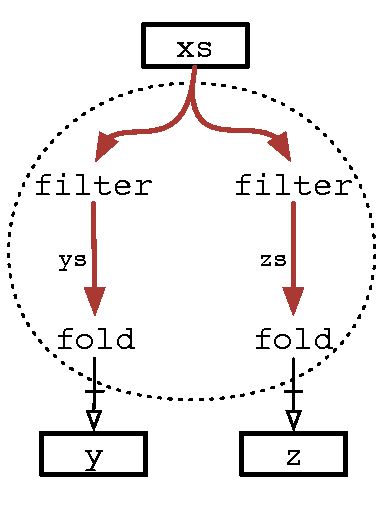
\includegraphics[scale=0.5]{copy/03-body/clustering/figures/ex4-concestors.pdf}
\end{center}
\end{minipage}
\caption{Program \Hs/sumPartition/ with clustering diagram}
\label{clustering:f:concestors}
\end{figure}

\begin{listing-c}[float,label=figs/clustering/sumPartition-c,caption=Unfused imperative implementation of \Hs/sumPartition/ with colour-coded iteration sizes]
void sumPartition(int* xs, size_t xs_length, int* out_y, int* out_z)
{
    // ys = filter ($>0$) xs
    int* ys = malloc(sizeof(int) * xs_length);
    size_t ys_length = 0;
    for (size_t i = 0; i != xs_length; ++i) {
        if (xs[i] > 0) ys[ys_length++] = xs[i];
    }

    // zs = filter ($<0$) xs
    int* zs = malloc(sizeof(int) * xs_length);
    size_t zs_length = 0;
    for (size_t i = 0; i != xs_length; ++i) {
        if (xs[i] < 0) zs[zs_length++] = xs[i];
    }

    // y = fold (+) 0 ys
    int y = 0;
    for (size_t i = 0; %\colorbox{purple!10}{\tt{i != ys\_length}}%; ++i) {
        y += ys[i];
    }
    *out_y = y;

    // z = fold (+) 0 zs
    int z = 0;
    for (size_t i = 0; %\colorbox{blue!10}{\tt{i != zs\_length}}%; ++i) {
        z += zs[i];
    }
    *out_z = z;

    free(ys);
    free(zs);
}
\end{listing-c}
\begin{listing-c}[float,label=figs/clustering/sumPartition-c-part,caption=Partially fused imperative implementation of \Hs/sumPartition/ with colour-coded iteration sizes]
void filter2(int* xs, size_t xs_length, int* out_y, int* out_z)
{
    // ys = filter ($>0$)  xs
    // y  = fold   (+) 0   ys
    int y = 0;
    for (size_t i = 0; %\colorbox{green!10}{\tt{i != xs\_length}}%; ++i) {
        if (xs[i] > 0) y += xs[i];
    }
    *out_y = y;

    // zs = filter ($<0$)  xs
    // z  = fold   (+) 0   zs
    int z = 0;
    for (size_t i = 0; %\colorbox{green!10}{\tt{i != xs\_length}}%; ++i) {
        if (xs[i] < 0) z += xs[i];
    }
    *out_z = z;
}
\end{listing-c}

We use the ancestor transducers to determine determine whether two combinators of different iteration sizes may be fused together.
\Cref{clustering:f:concestors} shows the \Hs/sumPartition/ example, which performs two filters over the same array, and computes the sum of each filter's output array.
The unfused imperative version, shown in \cref{figs/clustering/sumPartition-c}, performs each operation as a separate loop.
The last two loops compute the sums.
If we look at these two loops in isolation, the relationship between the two loop iteration sizes \Hs/ys_length/ and \Hs/zs_length/ is unknown, and it is not possible to fuse the two loops together without introducing excessively complicated control-flow.
The relationship between the two loop iteration sizes becomes clear when we consider each sum's parent transducer, which for the \Hs/y/ sum is the filter that produces \Hs/ys/, and for the \Hs/z/ sum is the filter that produces \Hs/zs/.
\Cref{figs/clustering/sumPartition-c-part} shows a partially fused imperative version, where each sum is fused with its parent transducer.
In this partially fused version, the two sums are still computed in separate loops, but both loops use the same iteration size.
Fusing these two loops together is trivial.

The key insight from this example is that two combinators of different iteration sizes may be fused together if each combinator is fused with its parent transducer, and the two parent transducers are also fused together.
If the two parent transducers also have different iteration sizes, their respective parent transducers must also be fused together.
In this case, we skip the parent transducers, and look directly at the closest pair of ancestor transducers with the same iteration size as each other.


\begin{figure}
% \begin{tabbing}
% MMMM \= M \= M \= M \= \kill
% $parents$ \> $:$ \> $binds \to name \to name \to \{name \times name\}$ \\
% $parents(bs, a, b)$ \\
%         \> $|$ \> $\iiter_{\Gamma,C}(bs(a)) == \iiter_{\Gamma,C}(bs(b))$ \\
%         \>     \>                      \> $=$ \> $\{(a, b)\}$ \\
%         \> $|$ \> otherwise            \\
%         \>     \>                      \> $=$    \> $\{ parents(bs, a', b) ~|~ a' \in trans(bs, a) \} $      \\
%         \>     \>                      \> $\cup$ \> $\{ parents(bs, a, b') ~|~ b' \in trans(bs, b) \} $  \\
% \end{tabbing}
% changed to return optional single closest parents:
%
\begin{tabbing}
MMMM \= M \= M \= M \= MMMM \= M \= \kill
$\concestors$ \> $:$ \> $\{\bind\} \to \name \to \name \to (\name \times \name)_\bot$ \\
$\concestors(bs, a, b)$ \\
        \> $|$ \> $(p_a,p_b,d) \in \concestors'(bs,a,b)$ \\
        \>     \>                      \> $=$ \> $\{(a, b)\}$ \\
        \> $|$ \> otherwise \\
        \>     \>                      \> $=$    \> $\bot$ \\
\\
$\concestors'$ \> $:$ \> $\{\bind\} \to \name \to \name \to (\name \times \name \times \mathbb{N})_\bot$ \\
$\concestors'(bs, a, b)$ \\
        \> $|$ \> $\iiter_{\Gamma,C}(bs(a)) == \iiter_{\Gamma,C}(bs(b))$ \\
        \>     \>                      \> $=$ \> $\{(a, b, 0)\}$ \\
        \> $|$ \> $a' \in \trans(bs,a),~ p_a \in \concestors'(bs,a',b)$ \\
        \> $,$ \> $b' \in \trans(bs,b),~ p_b \in \concestors'(bs,a,b')$ \\
        \>     \>                      \> $=$ \> $\mi{increment}(\mi{closest}(p_a, p_b))$ \\
        \> $|$ \> $a' \in \trans(bs,a),~ p_a \in \concestors'(bs,a',b)$ \\
        \>     \>                      \> $=$ \> $\mi{increment}(p_a)$ \\
        \> $|$ \> $b' \in \trans(bs,b),~ p_b \in \concestors'(bs,a,b')$ \\
        \>     \>                      \> $=$ \> $\mi{increment}(p_b)$ \\
        \> $|$ \> otherwise            \\
        \>     \>                      \> $=$    \> $\bot$
\\
\\
$\mi{closest}$ \> $:$ \> $(\name \times \name \times \mathbb{N}) \to (\name \times \name \times \mathbb{N}) \to (\name \times \name \times \mathbb{N})$ \\
$\mi{closest}((l_a,l_b,l_d), (r_a,r_b,r_d))$ \\
        \> $|$ \> $l_d \le r_d$ \> \> \> $=$ \> $(l_a,l_b,l_d)$ \\
        \> $|$ \> otherwise     \> \> \> $=$ \> $(r_a,r_b,r_d)$ \\
\\
$\mi{increment} :$ \> \> $(\name \times \name \times \mathbb{N}) \to (\name \times \name \times \mathbb{N})$ \\
$\mi{increment}((a,b,d)) = (a,b,d+1)$ \\
\end{tabbing}

\caption{Finding the compatible concestors, or most recent common ancestors with the same iteration size}
\label{fig:clustering:concestors}
\end{figure}

\Cref{fig:clustering:concestors} defines the $\concestors$ function, which finds the pair of most recent common ancestor transducers such that both ancestors have the same iteration size.
In the field of biological systematics, the term \emph{concestor} is defined as the most recent common ancestor; here, we define the \emph{compatible concestors} of a transducer to be the pair of most recent common ancestors with the same iteration size.
In the definition of the $\concestors$ function, we use the syntax $(name \times name)_\bot$ to denote an optional pair of names.
Two combinators $a$ and $b$ of different iteration size may be fused together only if they have compatible concestors $(c, d) \in \concestors(a,b)$, and the combinators and their compatible concestors are also fused together.
That is, in order for $a$ and $b$ to be fused together, $c$ and $d$ must be fused, $a$ and $c$ must be fused, and $d$ and $b$ must be fused.
If the two combinators have the same iteration size, the two compatible concestors will be the combinators themselves, and the above requirements for fusing different sized combinators are trivially satisfied, since a combinator is always fused with itself.

The definition of $\concestors'$ returns the pair of compatible concestors as well as the distance, determined by counting how many other ancestor transducers there are between the combinator and the compatible concestors.
The $\mi{closest}$ function compares the distances of two pairs of compatible concestors and chooses the closest pair.
The $\mi{increment}$ function increases the distance by one.

The $\trans$ function returns only the direct parent transducer, but a single combinator can have multiple ancestor transducers.
For a pair of combinators with multiple ancestor transducers, there may be multiple compatible common ancestors, but there can only be one pair of \emph{most recent} compatible common ancestors (compatible concestors), because of the tree structure of ancestor transducers.
In general, a pair of differently-sized combinators could be fused together if \emph{any} pair of compatible common ancestors are fused together with the combinators.
Because fusing the combinators with any pair of compatible common ancestors requires fusing with the compatible concestors as well, it is sufficient to require the pair of combinators to be fused with just the compatible concestors.

% Because each node has at most one transducer, and each transducer introduces a unique output size, the graph of ancestors forms a tree rather than a directed acyclic graph.
% A pair of nodes can have at most one most recent compatible common ancestor transducers, because each node has at most one transducer, and each transducer introduces a unique output size.
% This means that the ancestors are defined as a tree, rather than a directed acyclic graph, and each pair of nodes has a single common ancestor transducer.
% Two nodes cannot have the same iteration size if they have different parent transducers.
% A pair of nodes can have at most one pair of compatible concestors because each transducer has a unique output size.
% This means that, for two ancestor transducers to have the same iteration size, 

% Intuitively, a pair of nodes can have at most one pair of compatible concestors, because the transducers form a total ordering, and 
% The \emph{sole transducers} lemma ensures that a pair of nodes can have at most one pair of compatible concestors.
% If two nodes have a pair compatible concestors, it is unique, thanks to the \emph{sole transducers} lemma.
% To fuse a combinator with a particular ancestor, we must also fuse the combinator with all the nodes in the path between the combinator and its ancestor.
% In the definition of $\concestors$, we find the closest ancestors because it allows the most fusion; finding the furthest ancestors would be more restrictive, as it would also require fusing the inputs with any other ancestor transducers between the input combinators and the furthest ancestors.

\begin{haskell}[float,label=figs/clustering/normalize2-sizeinf,caption=Normalize2 function]
normalize2 :: Array Int -> (Array Int, Array Int)
normalize2 xs
 = let sum1 = fold   (+)  0   xs
       gts  = filter (>   0)  xs
       sum2 = fold   (+)  0   gts
       ys1  = map    (/ sum1) xs
       ys2  = map    (/ sum2) xs
   in (ys1, ys2)
\end{haskell}

The \Hs/normalize2/ example from earlier is repeated in \cref{figs/clustering/normalize2-sizeinf}.
In this example, \Hs@sum1@ consumes the input \Hs/xs/, while \Hs@sum2@ consumes the output of the filter \Hs/gts/, which in turn consumes the input \Hs/xs/.
The two folds have different iteration sizes, and their compatible concestors are $\concestors(\Hs@sum1@, \Hs@sum2@) = (\Hs@sum1@, \Hs@gts@)$.
The compatible concestors \Hs/sum1/ and \Hs/gts/ both consume the input \Hs/xs/ and have the same iteration size.
In order for \Hs@sum1@ and \Hs@sum2@ to be fused together, we require that: \Hs@sum1@ and \Hs@gts@ are fused together; \Hs@sum1@ and \Hs@sum1@ are fused together, which is trivial as fusion is reflexive;  and \Hs@gts@ and \Hs@sum2@ are fused together.
